\documentclass[tikz,border=4pt]{standalone}

\usepackage[T1]{fontenc}
\usepackage{libertine}
\usepackage{inconsolata}
\usepackage{newtxmath}
\usetikzlibrary{arrows.meta,calc}

\definecolor{graphink}{HTML}{263238}
\definecolor{orderfill}{HTML}{F5F1EA}
\definecolor{orderline}{HTML}{8C7256}
\definecolor{userfill}{HTML}{EEF4F7}
\definecolor{userline}{HTML}{557A8A}
\definecolor{relcolor}{HTML}{315F78}

\begin{document}
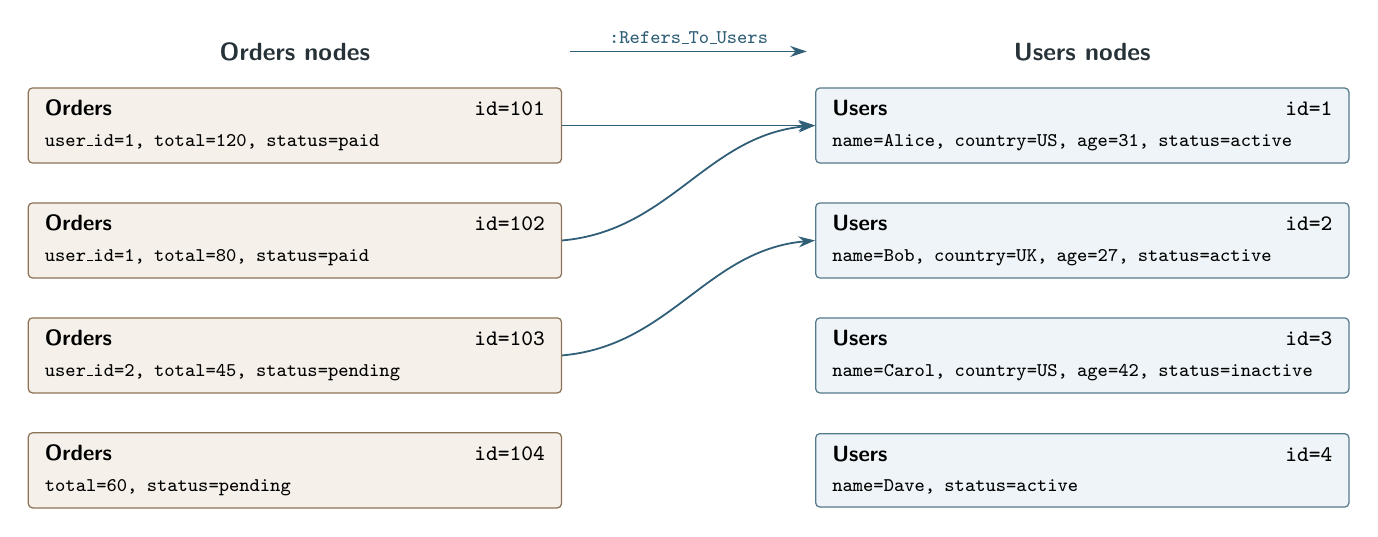
\begin{tikzpicture}[
  card/.style={
    draw=graphink!72,
    line width=0.45pt,
    rounded corners=1.5pt,
    text width=6.35cm,
    minimum height=0.84cm,
    inner xsep=6pt,
    inner ysep=4.5pt,
    align=left
  },
  order/.style={card, fill=orderfill, draw=orderline},
  user/.style={card, fill=userfill, draw=userline},
  heading/.style={font=\sffamily\bfseries\small, text=graphink},
  relationship/.style={
    -{Stealth[length=2.1mm,width=1.4mm]},
    draw=relcolor,
    line width=0.65pt
  },
  typekey/.style={
    font=\ttfamily\scriptsize,
    text=relcolor,
    fill=white,
    inner xsep=3pt,
    inner ysep=1.5pt
  }
]

\node[heading] at (0,3.12) {Orders nodes};
\node[heading] at (10.00,3.12) {Users nodes};
\draw[relationship] (3.50,3.12) --
  node[typekey,above=1pt] {:Refers\_To\_Users} (6.50,3.12);

\node[order] (o101) at (0,2.18)
  {\sffamily\bfseries\footnotesize Orders\hfill\ttfamily\footnotesize id=101\\[-1pt]
   \ttfamily\scriptsize user\_id=1, total=120, status=paid};
\node[order] (o102) at (0,0.72)
  {\sffamily\bfseries\footnotesize Orders\hfill\ttfamily\footnotesize id=102\\[-1pt]
   \ttfamily\scriptsize user\_id=1, total=80, status=paid};
\node[order] (o103) at (0,-0.74)
  {\sffamily\bfseries\footnotesize Orders\hfill\ttfamily\footnotesize id=103\\[-1pt]
   \ttfamily\scriptsize user\_id=2, total=45, status=pending};
\node[order] (o104) at (0,-2.20)
  {\sffamily\bfseries\footnotesize Orders\hfill\ttfamily\footnotesize id=104\\[-1pt]
   \ttfamily\scriptsize total=60, status=pending};

\node[user] (u1) at (10.00,2.18)
  {\sffamily\bfseries\footnotesize Users\hfill\ttfamily\footnotesize id=1\\[-1pt]
   \ttfamily\scriptsize name=Alice, country=US, age=31, status=active};
\node[user] (u2) at (10.00,0.72)
  {\sffamily\bfseries\footnotesize Users\hfill\ttfamily\footnotesize id=2\\[-1pt]
   \ttfamily\scriptsize name=Bob, country=UK, age=27, status=active};
\node[user] (u3) at (10.00,-0.74)
  {\sffamily\bfseries\footnotesize Users\hfill\ttfamily\footnotesize id=3\\[-1pt]
   \ttfamily\scriptsize name=Carol, country=US, age=42, status=inactive};
\node[user] (u4) at (10.00,-2.20)
  {\sffamily\bfseries\footnotesize Users\hfill\ttfamily\footnotesize id=4\\[-1pt]
   \ttfamily\scriptsize name=Dave, status=active};

\draw[relationship] (o101.east) -- (u1.west);
\draw[relationship] (o102.east) to[out=5,in=185] (u1.west);
\draw[relationship] (o103.east) to[out=5,in=185] (u2.west);

\end{tikzpicture}
\end{document}
